\setmodule{9}

%BEGIN_FOLD % ====>>_____ Занятие 1 _____<<====
\begin{class}[number=1]
		%G111M6L1 L2
		%\item Площадь грани прямоугольного параллелепипеда равна \( 15 \). Ребро, перпендикулярное этой грани, равно \(3\). Найдите объем параллелепипеда.
		%\item Три ребра прямоугольного параллелепипеда, выходящие из одной вершины, равны \(4, 6, 9\). Найдите ребро равновеликого ему куба.
		%\item Два ребра прямоугольного параллелепипеда, выходящие из одной вершины, равны \(3\) и \(4\). Площадь поверхности этого параллелепипеда равна \(94\). Найдите третье ребро, выходящее из той же вершины.
		%\item Объем прямоугольного параллелепипеда равен \(24\). Одно из его ребер равно \(3\). Найдите площадь грани параллелепипеда, перпендикулярной этому ребру.
		%\item Прямоугольный параллелепипед описан около сферы радиуса \(1\). Найдите его площадь поверхности.
		%\item Диагональ куба равна \( 2\sqrt{3} \). Найдите объем куба и площадь его поверхности.
		%\item Объем первого куба в \( 8 \) раз больше объема второго куба. Во сколько раз площадь поверхности первого куба больше площади поверхности второго куба?
		%\item Найдите площадь боковой поверхности правильной шестиугольной призмы, сторона основания которой равна \( 5 \), а высота  --- \( 10 \).
		%\item Дан куб \( ABCDA_1B_1C_1D_1 \). Площадь четырехугольника \( ABC_1D_1 \) равна \( 4\sqrt{2} \). Найдите площадь поверхности куба.
		%\item 
		%\begin{minipage}[t]{\bodywidth}
		%	В правильной треугольной пирамиде \(SABC\) с вершиной \(S\) биссектрисы треугольника \(ABC\) пересекаются в точке \(O\). Площадь треугольника \(ABC\) равна \(2\); объем пирамиды равен \(6\). Найдите длину отрезка \(OS\).
		%\end{minipage}
		%\hspace{0.02\linewidth}
		%\begin{minipage}[t]{\picwidth}
		%	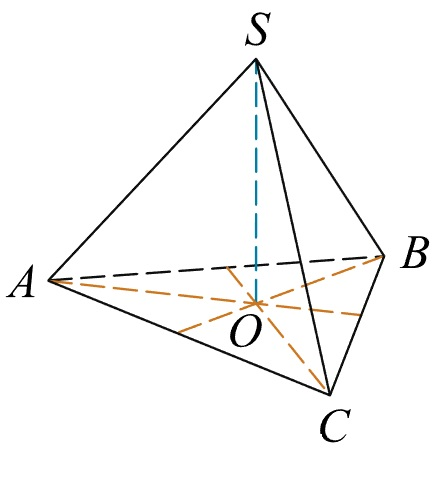
\includegraphics[align=t, width=\linewidth]{\picpath/G111M6L1-1}
		%\end{minipage}
		%\item В правильной четырехугольной пирамиде \(SABCD\) точка \(O\) --- центр основания, \(S\) --- вершина, \(SO=15, BD=16\). Найдите боковое ребро \(SA\).
		%
		%\item 
		%\begin{minipage}[t]{\bodywidth}
		%	В правильной треугольной пирамиде \(SABC\) точка \(M\) --- середина ребра \(AB\), \(S\) --- вершина. Известно, что \(BC = 3\), а площадь боковой поверхности пирамиды равна \(45\). Найдите длину отрезка \(SM\).
		%\end{minipage}
		%\hspace{0.02\linewidth}
		%\begin{minipage}[t]{\picwidth}
		%	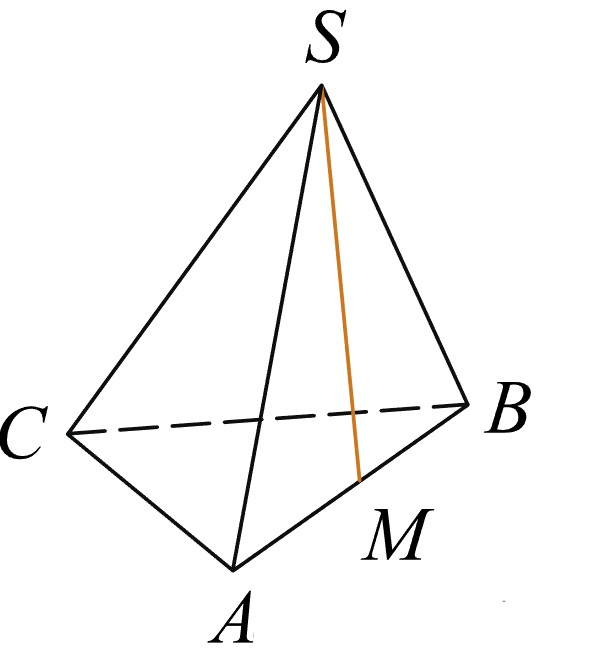
\includegraphics[align=t, width=\linewidth]{\picpath/G111M6L1-2}
		%\end{minipage}
		%\item Объем параллелепипеда \(ABCDA_1B_1C_1D_1\) равен \(9\). Найдите объем треугольной пирамиды \(ABCA_1\).
		%\item Во сколько раз увеличится объем правильного тетраэдра, если все его ребра увеличить в два раза?
		%\item В треугольнике \(ABC\) \(AB = 10, AC = BC\), высота \(AH = 8\). Найдите \(\cos{BAC}\).
		%\item В треугольнике со сторонами \(9\) и \(6\) проведены высоты к этим сторонам. Высота, проведённая к первой из этих сторон, равна \(4\). Чему равна высота, проведённая ко второй стороне?
		%\item Площадь параллелограмма \(ABCD\) равна \(24\). Точка \(M\) --- середина стороны \(BC\). Найдите площадь трапеции \(AMCD\).
		%\item 
		%\begin{minipage}[t]{\bodywidth}
		%	На рисунке изображен многогранник, все двугранные углы многогранника прямые. Найдите квадрат расстояния между вершинами \(B_2\) и \(D_3\) .
		%\end{minipage}
		%\hspace{0.02\linewidth}
		%\begin{minipage}[t]{\picwidth}
		%	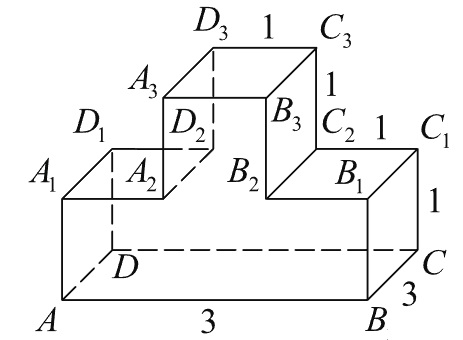
\includegraphics[align=t, width=\linewidth]{\picpath/G101M5L6-2}
		%\end{minipage}
		%\item 
		%\begin{minipage}[t]{\bodywidth}
		%	На рисунке изображен многогранник, все двугранные углы многогранника прямые. Найдите его объём и площадь поверхности.
		%\end{minipage}
		%\hspace{0.02\linewidth}
		%\begin{minipage}[t]{\picwidth}
		%	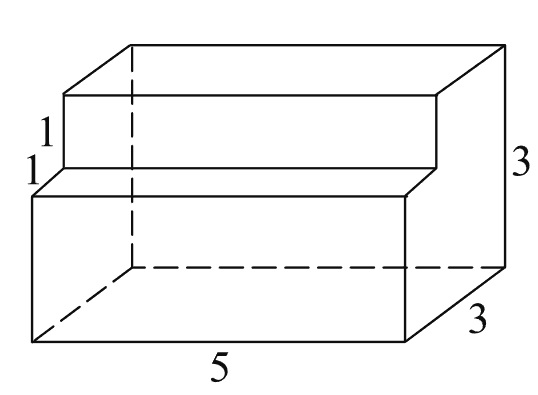
\includegraphics[align=t, width=\linewidth]{\picpath/G101M5L7-2}
		%\end{minipage}
		\begin{definit}
			Угол между пересекающимися плоскостями --- это наименьший из двугранных углов, образованных этими плоскостями.
			Угол между плоскостями равен углу между прямыми, соответственно перпендикулярными эти плоскостям.
		\end{definit}
		\begin{definit}
			Если одну из плоскостей заменить на параллельную, то полученный угол будет равен данному.
		\end{definit}
	\begin{listofex}
		%С27 1-3
		\item Дан куб \(ABCDA_1B_1C_1D_1\). Найдите угол между плоскостями:
		\begin{tasks}(2)
			\task \( BCC_1 \) и \( ABC_1 \);
			\task \( ABC \) и \( CB_1D_1 \);
			\task \( BA_1C_1 \) и \( AB_1D_1 \);
			\task \( ABC_1 \) и \( BCD_1 \).
		\end{tasks}
		\item Дан правильный тетраэдр \(ABCD\). Точки \(K\) и \(M\) --- середины рёбер \(BD\) и \(CD\) соответственно. Найдите углы между плоскостями:
		\begin{tasks}(3)
			\task \( AKC \) и \( ABD \);
			\task \( AMB \) и \( ABC \);
			\task \( AKM \) и \( ABC \).
		\end{tasks}
		\item Дана правильная четырёхугольная пирамида \(SABCD\) с вершиной \(S\). Все рёбра пирамиды равны, \(E\) --- середина бокового ребра \(SC\). Найдите углы между плоскостями:
		\begin{tasks}(3)
			\task \( SAD \) и \( SBC \);
			\task \( ABC \) и \( SCD \);
			\task \( ABC \) и \( BDE \).
			%\task \( BSC \) и \( DSC \).
			%\task \( ABE \) и \( ABC \).
		\end{tasks}
	\end{listofex}
	\begin{definit}
		Углом между прямой и плоскостью называется угол между прямой и её ортогональной проекцией на плоскость.
	\end{definit}
	\begin{listofex}[resume]
		%c45 1-2
		\item Дан куб \(ABCDA_1B_1C_1D_1\). Найдите углы:
		\begin{tasks}(1)
			\task между прямой \( AC_1 \) и плоскостью \(BDD_1 \);
			\task между прямой \(  AB\) и плоскостью \( CB_1D_1\);
			\task между прямой \( DD_1 \) и плоскостью \( ACB_1\);
			\task между прямой \( AC \) и плоскостью \( BCD_1\);
		\end{tasks}
		\item Дан правильный тетраэдр \(ABCD\). Точки \(K, M\) и \(N\) --- середины рёбер \(BD, AB\) и \(AC\) соответственно. Найдите углы:
		\begin{tasks}(1)
			\task между прямой \( CD \) и плоскостью \(ABD \);
			\task между прямой \(  DM\) и плоскостью \( ADC \);
			\task между прямой \( KN \) и плоскостью \( ADC\);
			\task между прямой \( BD \) и плоскостью \( KMN\);
		\end{tasks}
	\end{listofex}
\end{class}
%END_FOLD

%BEGIN_FOLD % ====>>_____ Занятие 2 _____<<====
\begin{class}[number=2]
	\begin{listofex}
		%c45 1-2
		\item Дан куб \(ABCDA_1B_1C_1D_1\). Найдите углы:
		\begin{tasks}(1)
			\task между прямой \( AC_1 \) и плоскостью \(BDD_1 \);
			\task между прямой \(  AB\) и плоскостью \( CB_1D_1\);
			\task между прямой \( DD_1 \) и плоскостью \( ACB_1\);
			\task между прямой \( AC \) и плоскостью \( BCD_1\);
		\end{tasks}
		\item Дан правильный тетраэдр \(ABCD\). Точки \(K, M\) и \(N\) --- середины рёбер \(BD, AB\) и \(AC\) соответственно. Найдите углы:
		\begin{tasks}(1)
			\task между прямой \( CD \) и плоскостью \(ABD \);
			\task между прямой \(  DM\) и плоскостью \( ADC \);
			\task между прямой \( KN \) и плоскостью \( ADC\);
			\task между прямой \( BD \) и плоскостью \( KMN\);
		\end{tasks}
		\item Дан правильный тетраэдр \(ABCD\). Точки \(K\) и \(M\) --- середины рёбер \(BD\) и \(CD\) соответственно. Найдите углы между плоскостями:
		\begin{tasks}(3)
			\task \( AKC \) и \( ABD \);
			\task \( AMB \) и \( ABC \);
			\task \( AKM \) и \( ABC \).
		\end{tasks}
		\item Дана правильная четырёхугольная пирамида \(SABCD\) с вершиной \(S\). Все рёбра пирамиды равны, \(E\) --- середина бокового ребра \(SC\). Найдите углы между плоскостями:
		\begin{tasks}(3)
			\task \( SAD \) и \( SBC \);
			\task \( ABC \) и \( SCD \);
			\task \( ABC \) и \( BDE \).
			%\task \( BSC \) и \( DSC \).
			%\task \( ABE \) и \( ABC \).
		\end{tasks}
	\end{listofex}
\end{class}
%END_FOLD

%BEGIN_FOLD % ====>>_ Домашняя работа 1 _<<====
\begin{homework}[number=1]
	\begin{listofex}
		\item Дана правильная четырёхугольная пирамида \(SABCD\) с вершиной \(S\). Все рёбра пирамиды равны, \(M\) --- середина бокового ребра \(SD\), \(E\) --- середина бокового ребра \(SC\).Найдите углы:
		\begin{tasks}
			\task между прямой \(AM\) и плоскостью \(ABC\);
			\task между прямой \(BD\) и плоскостью \(BSC\);
			\task между прямой \(BM\) и плоскостью \(ASD\);
			\task между прямой \(SA\) и плоскостью \(CSD\);
			\task между плоскостями \( BSC \) и \( DSC \);
			\task между плоскостями \( ABE \) и \( ABC \).
		\end{tasks}
	\end{listofex}
\end{homework}
%END_FOLD

%BEGIN_FOLD % ====>>_____ Занятие 3 _____<<====
\begin{class}[number=3]
	\begin{listofex}
		%с27 6
		\item Дана правильная шестиугольная пирамида \(SABCDEF\) с вершиной \(S\). Боковое ребро вдвое больше стороны основания. Найдите углы между плоскостями:
		\begin{tasks}(2)
			\task \( ABC \) и \(SEF\)
			\task \( SBD \) и \(ABC\)
			%\task \( SBC \) и \(SEF\)
			%\task \( SAF \) и \(SBC\)
		\end{tasks}
		%C28 3.1
		\item Основание пирамиды совпадает с одной из граней куба, а вершина --- с центром противоположной грани.
		\begin{tasks}
			\task Докажите, что пирамида правильная.
			\task Найдите угол между плоскостями её соседних боковых граней.
		\end{tasks}
		%C46 6
		\item Дана правильная шестиугольная пирамида \(SABCDEF\) с вершиной \(S\). Сторона основания равна \(1\), а боковое ребро равно \(2\). Найдите углы:
		\begin{tasks}
			\task между прямой \(BC\) и плоскостью \(ASF\)
			\task между прямой \(SA\) и плоскостью \(BSC\)
			%\task между прямой \(AB\) и плоскостью \(BSC\)
			%\task между прямой \(AC\) и плоскостью \(CSD\)
		\end{tasks}
		%c46 N 5.1
		\item Основание треугольной пирамиды \(DABC\) --- прямоугольный треугольник \(ABC\) \(\angle C = 90 \degree\). Высота пирамиды проходит через точку \(C\).
		\begin{tasks}
			\task Докажите, что противоположные рёбра пирамиды попарно перпендикулярны.
			\task Найдите углы, которые образуют боковые рёбра \(DA\) и \(DB\) с плоскостью основания, если \(AC =15\), \(BC =20\), а угол между плоскостями \(ABC\) и \(ABD\) равен \(45\degree\).
		\end{tasks}
	\end{listofex}
\end{class}
%END_FOLD

%BEGIN_FOLD % ====>>_____ Занятие 4 _____<<====
\begin{class}[number=4]
	\begin{listofex}
		%с28 N 3.2
		\item Дана правильная треугольная пирамида \(DABC\) с вершиной \(D\). Точка \(M\) --- середина ребра \(AB\), \(N\) --- основание перпендикуляра, опущенного из точки \(M\) на прямую \(CD\).
		\begin{tasks}
			\task Докажите, что прямая \(MN\) перпендикулярна прямой \(AB\).
			\task Найдите угол между боковыми гранями пирамиды, если угол между боковым ребром и плоскостью основания равен \(60\degree \).
		\end{tasks}
		%с28 N 3.3
		\item Дана правильная четырёхугольная пирамида \(SABCD\) с вершиной \(S\). Точка \(O\) --- центр основания, \(K\) --- основание перпендикуляра, опущенного из точки \(O\) на прямую \(SC\).
		\begin{tasks}
			\task Докажите, что прямая \(OK\) перпендикулярна прямой \(BD\).
			\task Найдите двугранный угол при боковом ребре пирамиды, если угол между боковым ребром и плоскостью основания равен \(60\degree \).
		\end{tasks}
		%c46 N5.2
		\item Высота \(PC\) треугольной пирамиды \(PABC\) с вершиной \(P\) проходит через точку \(C\). Прямые \(PA\) и \(BC\) перпендикулярны.
		\begin{tasks}
			\task Докажите, что основание пирамиды --- прямоугольный треугольник.
			\task Найдите углы, которые образуют боковые рёбра \(PA\) и \(PB\) с плоскостью основания, если \(AC = 6\), \(BC = 8\), а расстояние от точки \(P\) до прямой \(AB\) равно \(5\).
		\end{tasks}
	\end{listofex}
\end{class}
%END_FOLD

%BEGIN_FOLD % ====>>_ Домашняя работа 2 _<<====
\begin{homework}[number=2]
	\begin{listofex}
		%с27 6
		\item Дана правильная шестиугольная пирамида \(SABCDEF\) с вершиной \(S\). Боковое ребро вдвое больше стороны основания. Найдите углы между плоскостями:
		\begin{tasks}(2)
			\task \( SBC \) и \(SEF\)
			\task \( SAF \) и \(SBC\)
		\end{tasks}
		%C46 6
		\item Дана правильная шестиугольная пирамида \(SABCDEF\) с вершиной \(S\). Сторона основания равна \(1\), а боковое ребро равно \(2\). Найдите углы:
		\begin{tasks}
			\task между прямой \(AB\) и плоскостью \(BSC\)
			\task между прямой \(AC\) и плоскостью \(CSD\)
		\end{tasks}
		\item 
		\begin{tasks}
			\task 
			\task 
		\end{tasks}
	\end{listofex}
\end{homework}
%END_FOLD

%BEGIN_FOLD % ====>>_____ Занятие 5 _____<<====
\begin{class}[number=5]
	\begin{listofex}
		\item Занятие 5
	\end{listofex}
\end{class}
%END_FOLD

%BEGIN_FOLD % ====>>_____ Занятие 6 _____<<====
\begin{class}[number=6]
	\begin{listofex}
		\item Занятие 6
	\end{listofex}
\end{class}
%END_FOLD

%BEGIN_FOLD % ====>>_ Домашняя работа 3 _<<====
\begin{homework}[number=3]
	\begin{listofex}
		\item Домашняя работа 3
	\end{listofex}
\end{homework}
%END_FOLD

%BEGIN_FOLD % ====>>_____ Занятие 7 _____<<====
\begin{class}[number=7]
	\title{Подготовка к проверочной}
	\begin{listofex}
		\item Занятие 7
	\end{listofex}
\end{class}
%END_FOLD

%BEGIN_FOLD % ====>>_ Проверочная работа _<<====
\begin{exam}
	\begin{listofex}
		\item Проверочная
	\end{listofex}
\end{exam}
%END_FOLD


%BEGIN_FOLD % ====>>_ Консультация _<<====
\begin{consultation}
	\begin{listofex}
		\item Вероятность того, что в случайный момент времени температура тела здорового человека окажется ниже чем \( 36,8\degree C \), равна \( 0,81 \). Найдите вероятность того, что в случайный момент времени у здорового человека температура окажется \( 36,8\degree C \) или выше.
		\item При изготовлении подшипников диаметром \( 67 \) мм вероятность того, что диаметр будет отличаться от заданного не больше, чем на \( 0,01 \) мм, равна \( 0,965 \). Найдите вероятность того, что случайный подшипник будет иметь диаметр меньше чем \( 66,99 \) мм или больше чем \( 67,01 \) мм.
		\item Вероятность того, что батарейка бракованная, равна \( 0,06 \). Покупатель в магазине выбирает случайную упаковку, в которой две таких батарейки. Найдите вероятность того, что обе батарейки окажутся исправными.
		\item Вероятность того, что новый электрический чайник прослужит больше года, равна \( 0,93 \). Вероятность того, что он прослужит больше двух лет, равна \( 0,87 \). Найдите вероятность того, что он прослужит меньше двух лет, но больше года.
		\item Из районного центра в деревню ежедневно ходит автобус. Вероятность того, что в понедельник в автобусе окажется меньше \( 18 \) пассажиров, равна \( 0,82 \). Вероятность того, что окажется меньше \( 10 \) пассажиров, равна \( 0,51 \). Найдите вероятность того, что число пассажиров будет от \( 10 \) до \( 17 \).
		\item Помещение освещается фонарём с двумя лампами. Вероятность перегорания лампы в течение года равна \( 0,3 \). Найдите вероятность того, что в течение года хотя бы одна лампа не перегорит.
		\item В магазине стоят два платёжных автомата. Каждый из них может быть неисправен с вероятностью \( 0,05 \) независимо от другого автомата. Найдите вероятность того, что хотя бы один автомат исправен.
		\item B июле \( 2022 \) года планируется взять кредит в банке на некоторую сум-
		му. Условия его возврата таковы:\\
		— каждый январь долг увеличивается на \( 20\% \) по сравнению с концом предыдущего года;\\
		— с февраля по июнь каждого года необходимо выплатить одним платежом часть долга.\\
		Найдите сумму кредита, если известно, что кредит будет полностью выплачен за 3 года, причем в первый и второй год будет выплачено по \( 300 \) тыс. руб., а в третий \( 417,6 \) тыс. руб.
		\item B июле \( 2026 \) года планируется взять кредит на пять лет в размере \( 3,3 \) млн руб. Условия его возврата таковы:\\
		— каждый январь долг будет возрастать на \( 20\% \) по сравнению с концом предыдущего года;\\
		— с февраля по июнь каждого года необходимо выплатить часть долга;\\
		— в июле \( 2027 \), \( 2028 \) и \( 2029 \) годах долг остается равен \( 3,3 \) млн руб.;\\
		— платежи в \( 2030 \) и \( 2031 \) годах должны быть равны;\\
		— к июлю \( 2031 \) года долг должен быть выплачен полностью.\\
		Найдите разницу между первым и последним платежами.
		\item a) Решите уравнение \( \sin2x=2\sin x + \sin \left( x+\dfrac{ 3\pi }{ 2 } \right)+1\) \\
		б) Найдите все корни этого уравнения, принадлежащие отрезку \( \left[ - 4\pi; -\dfrac{5\pi}{2} \right]  \)
		\item a) Решите уравнение \( \cos2x+0,5=\cos^2x \). \\
		б) Найдите все корни этого уравнения, принадлежащие отрезку \( \left[ -2\pi;-\dfrac{\pi}{2} \right]  \)
	\end{listofex}
\end{consultation}
%END_FOLD